\section{Fitting Natural Splines}
%
%
\begin{frame}
  Since we know that the solution to our optimization problem must be a natural cubic spline, we can restate the problem as a search over a smaller set of curves:
  \begin{block}{Problem: Unconstrained, Roughness Penalty}
    $$ f_{\lambda}^* = \argmin_{s} \left\{ \sum_i (x_i - s(x_i))^2 + \lambda \int (s'')^2 \mid s \in \natsplines \right\} $$
  \end{block}
\end{frame}
%
%
\begin{frame}
  This is actaully a huge simplification, because $\natsplines$ is an infinitely smaller set to search over than ``all curves with second derivatives''.
\end{frame}
%
%
\begin{frame}
  We can make the smallness of $\natsplines$ precise, because it is a vector space:
  $$ g, h \in \natsplines \implies g + h \in \natsplines $$
  It's easy to determine the dimension of $\natsplines$... 
\end{frame}
%
%
\begin{frame}
	\begin{figure}
    \includegraphics[scale=0.12]{first_part_of_spline}
	\end{figure}
  The leftmost section has two (linear) degrees of freedom, the slope and vertical position of the line.
\end{frame}
%
%
\begin{frame}
	\begin{figure}
    \includegraphics[scale=0.08]{middle_part_of_spline}
	\end{figure}
  The middle (cubic) sections have one degree of freedom each.  A general cubic has four, and we use:
  \begin{itemize}
    \item One to match the left endpint of this section with the right endpoint of the previous.
    \item One to match the first derivatives.
    \item One to match the second derivatives.
  \end{itemize}
\end{frame}
%
%
\begin{frame}
	\begin{figure}
    \includegraphics[scale=0.08]{last_cubic_part_of_spline}
	\end{figure}
  The final cubic section has zero degrees of freedom.  Again, the general cubic has four and we use::
  \begin{itemize}
    \item One to match the left endpint of this section with the right endpoint of the previous.
    \item One to match the first derivatives.
    \item One to match the second derivatives.
    \item One to ensure that the second derivative vanishes at the rightmost endpoint.
  \end{itemize}
\end{frame}
%
%
\begin{frame}
	\begin{figure}
    \includegraphics[scale=0.1]{last_part_of_spline}
	\end{figure}
  The final section has zero degrees of freedom.  A general line has two and we must use:
  \begin{itemize}
    \item One to match the left endpint of this section with the right endpoint of the previous.
    \item One to match the first derivatives.
  \end{itemize}
\end{frame}
%
%
\begin{frame}
  So altogether:
  $$ \dim \natsplines = 2 + \underbrace{1 + \cdots + 1}_{n-2 times} + 0 + 0 = n $$
\end{frame}
%
%
\begin{frame}
  The upshot is that $\natsplines$ has a basis.  That is, there is a (in fact, many) set(s) of $n$ \textbf{fixed and specific} splines, so that any spline can be written in \textbf{exactly one way} as a sum:
  $$ s = \sum_{i=1}^n \alpha_i \sigma_i $$
where each $\alpha_i$ is just a number and each $\sigma_i$ is a specific cubic spline in the basis.
\end{frame}
%
%
\begin{frame}
  Another way to think of a basis is as a fixed way of associating a vector of numbers to a natural spline:
  $$ s \mapsto (\alpha_1, \alpha_2, \ldots, \alpha_n) $$
And in the opposite way, a natural spline to a vector of real numbers:
  $$ (\alpha_1, \alpha_2, \ldots, \alpha_n) \mapsto \sum \alpha_i \sigma_i $$
\end{frame}
%
%
\begin{frame}
  There are many possible choices of basis, with varying properties that are convenient for different applications. 
\end{frame}
%
%
\begin{frame}
  \begin{columns}
    \column{.75\textwidth}
      \includegraphics[scale=0.12]{reinsch_basis}
    \column{.25\textwidth}
      For example, here we have plotted the Reinsch basis for the natural splines with knots at $\{ .1, .2, \ldots, .9\}$
  \end{columns}
\end{frame}
%
%
\begin{frame}
  \begin{columns}
    \column{.75\textwidth}
      \includegraphics[scale=0.12]{reinsch_basis}
    \column{.25\textwidth}
      The Reinsch basis is quite special, and working with it makes many properties of cubic splines much more apparent.
  \end{columns}
  
\end{frame}

\begin{frame}
  We can now break down our problem one step further, instead of focusing on finding the optimal spline, let's think in terms of the \textit{coefficients of that optimal spline when written in terms of a fixed basis}.
    $$ s_{\alpha} = \sum_{i=1}^{n} \alpha_i \sigma_i $$
    $$ f_{\lambda}^* = s_{\alpha} = \argmin_{\alpha} \left\{ \sum_i (x_i - s_{\alpha}(x_i))^2 + \lambda \int (s_{\alpha}'')^2 \right\} $$
\end{frame}
%
%
\begin{frame}
  The end is finally in sight, this has the distinct smell of a linear algebra problem. 
\end{frame}
%
%
\begin{frame}
  We can write the sum of squares term in matrix form by introducing:
  $$ \mathbf{\Sigma} = \left( \sigma_j (x_i) \right) $$
  This simply evaluates every spline in the basis at every knot, and so is square matrix.
\end{frame}
%
%
\begin{frame}
  The residual sum of squares term can be written in terms of the $\mathbf{\Sigma}$ matrix:
  $$ (\mathbf{y} - \mathbf{\Sigma} \mathbf{\alpha})^{t}(\mathbf{y} - \mathbf{\Sigma} \mathbf{\alpha})$$
\end{frame}
%
%
\begin{frame}
  As for the penalty term, if we carry through the squaring:
  $$ \int (s_{\alpha}'')^2 = \int \left( \sum_i \alpha_i \sigma_i'' \right)^2 = \sum_{i,j} \alpha_i \alpha_j \int \sigma_i'' \sigma_j'' $$
\end{frame}
%
%
\begin{frame}
  So with the square matrix:
  $$ \mathbf{\Omega} = \left( \int \sigma_i'' \sigma_j'' \right) $$
  the penalty term becomes:
  $$ \alpha^t \mathbf{\Omega} \alpha $$
\end{frame}
%
%
\begin{frame}
  The final problem in matrix form now looks like:
  \begin{block}{Problem: Matrix Form}
    $$\alpha^* = \argmin_{\alpha} \left\{ (\mathbf{y} - \mathbf{\Sigma} \mathbf{\alpha})^{t}(\mathbf{y} - \mathbf{\Sigma} \mathbf{\alpha}) + \lambda \alpha^t \mathbf{\Omega} \alpha \right\} $$ 
  \end{block}
  Which can be solved by taking the gradient, setting to zero, and solving the resulting linear equation:
  $$ \alpha = ( \mathbf{\Sigma}^t \mathbf{\Sigma} + \lambda \mathbf{\Omega} )^{-1} \mathbf{\Sigma}^t y $$
\end{frame}
%
%
\begin{frame}
  The matrix form looks a lot like ridge regression:
  \begin{block}{Problem: Ridge Regression}
    $$ \beta = \argmin_{\beta} \left\{ (\mathbf{y} - X \beta)^t (\mathbf{y} - C \beta) + \lambda \beta^t \beta \right\} $$
 \end{block}
 Which has the solution:
 $$ \alpha = ( X^t X + \lambda I )^{-1} X^t y $$
 Ridge regression shrinks the parameters from the full linear regression fit towards zero.
\end{frame}
%
%
\begin{frame}
  By analogy, the roughness penalty shrinks the full interpolating spline fit in an intelegent way.  Essentially the ``high frequency'' terms in a basis are shrunk more than the ``low frequency'' terms, reducing the complexity of the interpolating spline.
\end{frame}
%
%
\begin{frame}
  The ``a basis'' in the previous slide is a special one: an eigenbasis of the quadratic form $\mathbf{\Omega}$.  Here's a picture of a few such eigenvectors (eigensplines) in that basis (taken from Hastie, Tibshirani and Friedman):
  \begin{figure}
    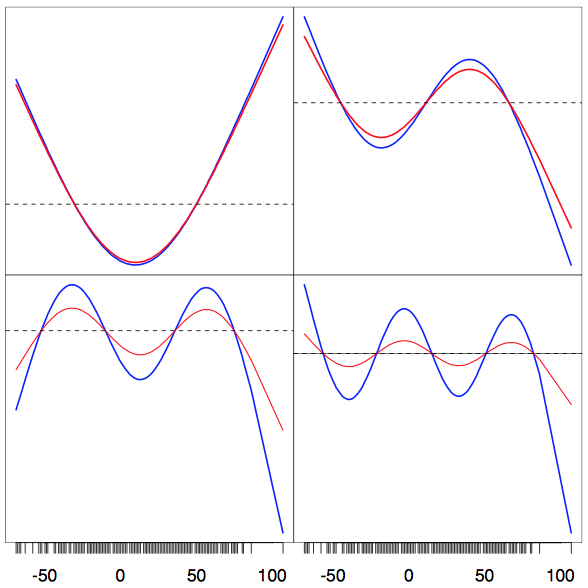
\includegraphics[scale=.5]{hastie_eigenvalues}
  \end{figure}
\end{frame}
